% This file was created by tikzplotlib v0.9.6.
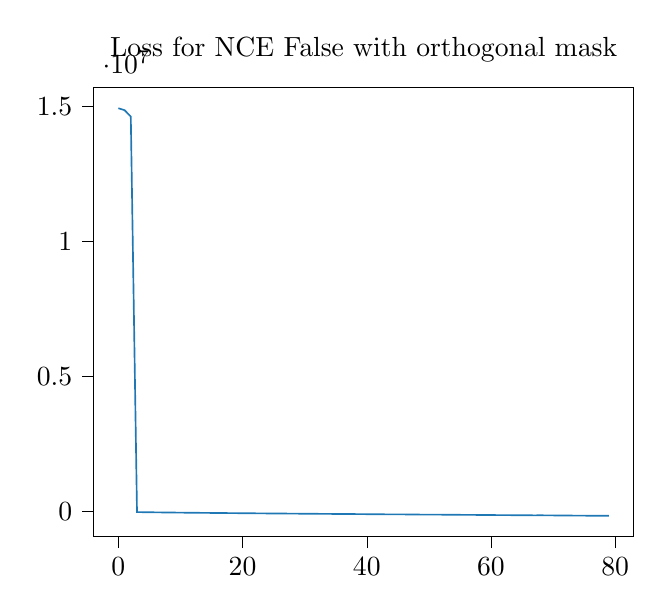
\begin{tikzpicture}

\definecolor{color0}{rgb}{0.12156862745098,0.466666666666667,0.705882352941177}

\begin{axis}[
tick align=outside,
tick pos=left,
title={Loss for NCE False with orthogonal mask},
x grid style={white!69.0196078431373!black},
xmin=-3.95, xmax=82.95,
xtick style={color=black},
y grid style={white!69.0196078431373!black},
ymin=-906312.213716807, ymax=15676596.7979696,
ytick style={color=black}
]
\addplot [semithick, color0]
table {%
0 14922828.2065293
1 14851322.0153235
2 14613628.1243846
3 -14924.0312438251
4 -18325.4300028998
5 -21526.0714124805
6 -24439.5292240158
7 -27215.2974540656
8 -29855.2113649352
9 -32400.6446478801
10 -34993.8804898312
11 -37333.903464459
12 -39746.8203947197
13 -41990.7105366933
14 -44087.6691429382
15 -46056.2093561942
16 -48171.1686182579
17 -50417.1724380575
18 -52264.1077266666
19 -54356.2635831562
20 -56468.47839116
21 -57976.144394764
22 -60414.5639933364
23 -62704.6239484305
24 -64425.4038137519
25 -66106.99281673
26 -68176.2359662242
27 -69720.824769196
28 -71281.3497486823
29 -73304.7512832187
30 -75357.1371885734
31 -77657.0046706549
32 -78713.9164210394
33 -81048.1241685911
34 -81963.8399462666
35 -83603.2805701209
36 -86133.3932952854
37 -87541.3213781795
38 -87975.2354536352
39 -90758.5584489338
40 -91946.4280692278
41 -94516.330204542
42 -95430.0163919909
43 -98004.1524679738
44 -99778.2208729671
45 -99757.6351703303
46 -100667.070211765
47 -102508.036159486
48 -105472.492962282
49 -108368.703798614
50 -108504.221207585
51 -109477.628041207
52 -109983.3324171
53 -113582.567708837
54 -115556.140089701
55 -116068.211990037
56 -117040.870646596
57 -118187.692409934
58 -120430.565149049
59 -122202.171431519
60 -124473.800338794
61 -125706.5250792
62 -125802.773463053
63 -128334.852060357
64 -130914.556999674
65 -132259.232989933
66 -132931.807576448
67 -135387.14694955
68 -133352.156514522
69 -136343.769820478
70 -137656.789977815
71 -141209.845412414
72 -143195.836710575
73 -143789.548614026
74 -144782.694850325
75 -146340.188417037
76 -149886.339763313
77 -149537.358239353
78 -152543.622276516
79 -149220.345394974
};
\end{axis}

\end{tikzpicture}
